\documentclass[12pt]{article}
\usepackage[ukrainian,shorthands=off]{babel}   % shorthands=off: символ " не активний (потрібно для міток "..." у TikZ всередині \zadtask)
\usepackage{fontspec}
% --- НАЛАШТУВАННЯ ШРИФТІВ ---
% Шрифти Schoolbook-*.otf лежать у корені проєкту. Шлях підбирається автоматично:
% ../ (компіляція з папки теми), ./ (корінь проєкту), ../../ (підпапки теми 28); інакше -- TeX Gyre Schola.
\newcommand{\nmtSchoolbook}[1]{\setmainfont{Schoolbook-Regular.otf}[
    Path = #1,
    BoldFont = Schoolbook-Bold.otf,
    ItalicFont = Schoolbook-Italic.otf,
    BoldItalicFont = Schoolbook-BoldItalic.otf
]}
\IfFileExists{../Schoolbook-Regular.otf}{\nmtSchoolbook{../}}{%
 \IfFileExists{./Schoolbook-Regular.otf}{\nmtSchoolbook{./}}{%
  \IfFileExists{../../Schoolbook-Regular.otf}{\nmtSchoolbook{../../}}{%
   \setmainfont{texgyreschola}[Extension=.otf, UprightFont=*-regular, BoldFont=*-bold, ItalicFont=*-italic, BoldItalicFont=*-bolditalic]}}}
\usepackage[italic]{mathastext}
\usepackage[a4paper,margin=1.8cm,bottom=2cm,top=2cm]{geometry}
\usepackage{amsmath,amssymb}
\usepackage{tikz}
\usepackage{pgfplots}
\pgfplotsset{compat=1.18}
\usepgfplotslibrary{fillbetween}
\usetikzlibrary{calc,patterns,angles,quotes,intersections,babel,3d,shapes.symbols,shapes.geometric,decorations.pathreplacing,shadings,arrows.meta,hobby}
\usepackage{xcolor,array,fancyhdr,enumitem,multicol}
\usepackage{colortbl,multirow,diagbox,needspace}
\usepackage{tcolorbox}
\tcbuselibrary{skins,breakable}
\usepackage[hidelinks]{hyperref}
% водяний знак; щоб зібрати без нього (версія для вчителів), перед \documentclass пишуть \def\nmtnowatermark{}
\ifdefined\nmtnowatermark\else
\usepackage[firstpage=false, text=@pvtr2525, scale=0.6, color=gray!12]{draftwatermark}
\fi

% --- АВТОСТИСКАННЯ: рисунок/сітка, ширша за колонку, масштабується до ширини колонки ---
\newsavebox{\nmtfitbox}
\newenvironment{nmtfit}{\begin{lrbox}{\nmtfitbox}}{\end{lrbox}%
  \ifdim\wd\nmtfitbox>\linewidth \resizebox{\linewidth}{!}{\usebox{\nmtfitbox}}\else\usebox{\nmtfitbox}\fi}
\let\nmtIncludegraphicsOrig\includegraphics
\renewcommand{\includegraphics}[2][]{\begin{nmtfit}\nmtIncludegraphicsOrig[#1]{#2}\end{nmtfit}}


\definecolor{mainGreen}{RGB}{34, 120, 64}
\definecolor{yearOrange}{RGB}{220, 100, 30}
\definecolor{yearcolor}{RGB}{220, 100, 30}
\definecolor{titleBg}{RGB}{225, 240, 220}
\definecolor{instrBg}{RGB}{255, 240, 220}
\definecolor{instrBorder}{RGB}{220, 150, 80}
\definecolor{headerblue}{RGB}{0, 102, 204}   % використовується в рисунках старої бази

\setlength{\parindent}{0pt}
\emergencystretch=1.5em

\pagestyle{fancy}
\fancyhf{}
\renewcommand{\headrulewidth}{0.4pt}
\renewcommand{\footrulewidth}{0.4pt}
\fancyhead[C]{\small\color{gray!80} Пробний НМТ № 1}
\fancyhead[R]{\small\color{mainGreen}\textbf{\href{https://t.me/pvtr2525}{@pvtr2525}}}
\fancyfoot[L]{\small\color{gray!80}\href{https://t.me/pvtr2525}{ТГ: @pvtr2525}}
\fancyfoot[C]{\small\color{gray!80}\thepage}
\fancyfoot[R]{\small\color{gray!80}НМТ з математики}

% --- ТАБЛИЦІ ВІДПОВІДЕЙ ---
% ширина клітинки = (ширина рядка - відступи) / 5: на всю сторінку це ~3 см, у minipage поруч із рисунком таблиця стискається;
% п'ять колонок |m{w}| мають 10 відступів \tabcolsep і 6 вертикальних ліній -- тоді таблиця рівно на \linewidth
\newlength{\nmtcellw}
\newcommand{\nmtSetCell}{\setlength{\nmtcellw}{\dimexpr(\linewidth-10\tabcolsep-6\arrayrulewidth)/5\relax}}
\newcommand{\answerTable}[5]{%
\par\nopagebreak\vspace{0.15cm}
\noindent\nmtSetCell
\begin{tabular}{|*{5}{>{\centering\arraybackslash}m{\nmtcellw}|}}
\hline
\rule[-0.15cm]{0pt}{0.6cm}\textbf{А} & \rule[-0.15cm]{0pt}{0.6cm}\textbf{Б} & \rule[-0.15cm]{0pt}{0.6cm}\textbf{В} & \rule[-0.15cm]{0pt}{0.6cm}\textbf{Г} & \rule[-0.15cm]{0pt}{0.6cm}\textbf{Д} \\
\hline
\rule[-0.2cm]{0pt}{0.75cm}#1 & \rule[-0.2cm]{0pt}{0.75cm}#2 & \rule[-0.2cm]{0pt}{0.75cm}#3 & \rule[-0.2cm]{0pt}{0.75cm}#4 & \rule[-0.2cm]{0pt}{0.75cm}#5 \\
\hline
\end{tabular}
\par\vspace{0.25cm}
}
\newcommand{\answerTableTall}[5]{%
\par\nopagebreak\vspace{0.15cm}
\noindent\nmtSetCell
\begin{tabular}{|*{5}{>{\centering\arraybackslash}m{\nmtcellw}|}}
\hline
\rule[-0.2cm]{0pt}{0.7cm}\textbf{А} & \rule[-0.2cm]{0pt}{0.7cm}\textbf{Б} & \rule[-0.2cm]{0pt}{0.7cm}\textbf{В} & \rule[-0.2cm]{0pt}{0.7cm}\textbf{Г} & \rule[-0.2cm]{0pt}{0.7cm}\textbf{Д} \\
\hline
\rule[-0.45cm]{0pt}{1.2cm}#1 & \rule[-0.45cm]{0pt}{1.2cm}#2 & \rule[-0.45cm]{0pt}{1.2cm}#3 & \rule[-0.45cm]{0pt}{1.2cm}#4 & \rule[-0.45cm]{0pt}{1.2cm}#5 \\
\hline
\end{tabular}
\par\vspace{0.25cm}
}
\newcommand{\instructionBox}[1]{%
\par\vspace{0.3cm}
\begin{tcolorbox}[colback=instrBg, colframe=instrBorder, boxrule=0.6pt, arc=2pt,
    left=8pt, right=8pt, top=4pt, bottom=4pt]
\centering\small\bfseries #1
\end{tcolorbox}
\par\vspace{0.15cm}
}
\newcommand{\sectionTitle}[1]{%
\par\vspace{0.4cm}
\begin{tcolorbox}[colback=titleBg, colframe=titleBg, boxrule=0pt, arc=8pt,
    halign=center, fontupper=\Large\bfseries\color{mainGreen}]
\hyphenpenalty=10000 \exhyphenpenalty=10000 #1
\end{tcolorbox}
\par\vspace{0.3cm}
}
\newcommand{\task}[2]{\noindent\textbf{#1.}\ \ #2\par\vspace{0.2cm}}
% --- НМТ-СТИЛЬ ПОЛЕ ВІДПОВІДІ ---
\newcommand{\nmtAnswerBox}{%
\par\nopagebreak\vspace{0.2cm}\noindent
Відповідь:\ \
\begin{tabular}{@{}*{4}{|>{\centering\arraybackslash}p{0.8cm}}|@{\hspace{0.1cm}\textbf{,}\hspace{0.1cm}}*{3}{|>{\centering\arraybackslash}p{0.8cm}}|@{}}
\hline
\rule[-0.2cm]{0pt}{0.7cm} & & & & & & \\
\hline
\end{tabular}
\par\vspace{0.3cm}
}
% --- СІТКА ДЛЯ МАТЧИНГУ ---
\newsavebox{\nmtgridbox}
\newcommand{\matchingGrid}{%
    \sbox{\nmtgridbox}{\matchingGridRaw}%
    \ifdim\wd\nmtgridbox>\linewidth \resizebox{\linewidth}{!}{\usebox{\nmtgridbox}}\else\usebox{\nmtgridbox}\fi}
\newcommand{\matchingGridRaw}{%
    \begingroup
    \renewcommand{\arraystretch}{1.15}
    \setlength{\tabcolsep}{4pt}
    \footnotesize
    \begin{tabular}{r|c|c|c|c|c|}
         \multicolumn{1}{c}{} & \multicolumn{1}{c}{\textbf{А}} & \multicolumn{1}{c}{\textbf{Б}} & \multicolumn{1}{c}{\textbf{В}} & \multicolumn{1}{c}{\textbf{Г}} & \multicolumn{1}{c}{\textbf{Д}} \\ \cline{2-6}
         \textbf{1} & \phantom{X} & \phantom{X} & \phantom{X} & \phantom{X} & \phantom{X} \\ \cline{2-6}
         \textbf{2} & & & & & \\ \cline{2-6}
         \textbf{3} & & & & & \\ \cline{2-6}
    \end{tabular}
    \endgroup
}
% --- ДОДАТКОВІ МАКРОСИ ЗБІРНИКА ---
\newcommand{\taskBlock}[1]{%
\par\vspace{0.45cm}
\noindent{\color{mainGreen}\rule{\linewidth}{0.8pt}}\par\vspace{0.12cm}
\noindent{\small\bfseries\color{mainGreen}#1}\par\vspace{0.25cm}
}
\newcounter{zad}
\newcommand{\zadtask}[1]{\stepcounter{zad}\noindent\textbf{\thezad.}\ \ #1\par\nopagebreak\vspace{0.2cm}}
\newcommand{\zadnum}{\stepcounter{zad}\textbf{\thezad.}\ \ }
\newcounter{ans}
\newcommand{\ansitem}[1]{\stepcounter{ans}\noindent\textbf{\theans.}\ #1\par\vspace{0.07cm}}
% мітка року: нерозривна, притиснута праворуч; якщо не вміщається -- праворуч на новому рядку
\newcommand{\nmtyear}[1]{\unskip\nobreak\finalhyphendemerits=0 \hfill\penalty100\hskip1em\hbox{}\nobreak\hfill{\small\color{yearOrange}\mbox{\rule{0pt}{2.3ex}(НМТ~#1)}}}
% --- МАКРОС КОРОТКОГО РОЗВ'ЯЗКУ ---
\newcommand{\solution}[1]{%
\par\vspace{0.12cm}
\begin{tcolorbox}[colback=titleBg!45, colframe=mainGreen!55, boxrule=0.4pt, arc=2pt,
    left=6pt, right=6pt, top=3pt, bottom=3pt, breakable]
\footnotesize\textbf{Короткий розв'язок.}\ #1
\end{tcolorbox}
\par\vspace{0.12cm}
}
% Розв'язки й відповіді (є до завдань НМТ-2026): \showsolutionstrue -- показати, \showsolutionsfalse -- сховати
\newif\ifshowsolutions
\showsolutionsfalse
% --- ЗАГОЛОВКИ З ПУНКТАМИ КЛІКАБЕЛЬНОГО ЗМІСТУ ---
\setcounter{tocdepth}{2}
\newcommand{\chapterTitle}[1]{%
\clearpage\phantomsection\addcontentsline{toc}{section}{#1}%
\sectionTitle{#1}}
\newcommand{\typeTitle}[1]{%
\needspace{6\baselineskip}%
\phantomsection\addcontentsline{toc}{subsection}{\quad #1}%
\par\vspace{0.3cm}
\noindent{\large\bfseries\color{yearOrange}#1}\par\vspace{0.08cm}
\noindent{\color{yearOrange}\rule{\linewidth}{0.4pt}}\par\nopagebreak\vspace{0.2cm}}
\raggedbottom
% усередині одного завдання сторінка не розривається: нерозривний вертикальний проміжок
% і нерозривна межа абзаців (умова ніколи не відділяється від варіантів, рисунка чи сітки)
\newcommand{\nbvspace}[1]{\nopagebreak\vspace{#1}}
\newcommand{\nmtnobreak}{\ifvmode\penalty10000 \fi}
% --- ЄДИНИЙ МАКЕТ ЗАВДАНЬ НА ВІДПОВІДНІСТЬ ---
% мітка в колонці сталої ширини, текст -- у parbox: продовження довгого рядка
% вирівнюється під текстом, а не під міткою; відступ між пунктами однаковий скрізь
\newlength{\nmtMatchLab}\setlength{\nmtMatchLab}{1.6em}
\newlength{\nmtMatchSep}\setlength{\nmtMatchSep}{0.28cm}
\newcommand{\matchHead}[1]{\par\noindent\textit{#1}\par\nopagebreak\vspace{0.2cm}}
% шаблонний заголовок стовпця зі старого макета -- лише коли завдання не має власного \matchHead
\makeatletter\newcommand{\nmtHeadUnless}[2]{\in@{\matchHead}{#1}\ifin@\else#2\fi}\makeatother
\newcommand{\matchItem}[2]{\par\noindent\makebox[\nmtMatchLab][l]{\textbf{#1}}%
\parbox[t]{\dimexpr\linewidth-\nmtMatchLab\relax}{\raggedright #2}\par\nopagebreak\vspace{\nmtMatchSep}}
\newcommand{\ansTheme}[1]{\par\vspace{0.25cm}\noindent{\bfseries\color{mainGreen}#1}\par\vspace{0.12cm}}
\newcommand{\ansType}[1]{\par\vspace{0.1cm}\noindent{\itshape\color{yearOrange}#1}\par\vspace{0.08cm}}

\graphicspath{{../1. Числа. Звичайні та десяткові дроби. Модуль числа/}{../10. Основи планіметрії/}{../11. Трикутники/}{../12. Паралелограм/}{../13. Прямокутник/}{../14. Квадрат/}{../15. Ромб/}{../16. Трапеція/}{../17. Коло, круг і їх елементи/}{../18. Координати і вектори на площині і в просторі. Рівняння кола/}{../19. Лінійні та квадратні нерівності. Системи лінійних нерівностей. Метод інтервалів/}{../2.відсотки, арифметичні задачі, подільність/}{../20. Функція та її властивості/}{../21.  Графіки елементарних функцій, їх побудова графіків функцій та їх перетворення/}{../22. Модульні  рівняння та нерівності/}{../23. Ірраціональні рівняння та нерівності/}{../24. Арифметична прогресія/}{../25. Геометрична прогресія/}{../26. Тригонометричні вирази/}{../27. Тригонометричні рівняння/}{../28. Показникова функція. Показникові рівняння/Показникові рівняння/}{../28. Показникова функція. Показникові рівняння/Показникові функція і вирази/}{../29. Показникові нерівності/}{../3. Степені. Одночлени. стандартний вигляд числа/}{../30. Логарифм. Логарифмічна функція/}{../31. Логарифмічні рівняння/}{../32. Логарифмічні нерівності/}{../33. Похідна/}{../34. Первісна/}{../35. Комбінаторика/}{../36. Теорія ймовірності/}{../37. Статистика/}{../38. Призма. Паралелепіпед. Куб/}{../39. Піраміда/}{../4.Многочлени. ФСМ/}{../40. Циліндр/}{../41. Конус/}{../42. Куля. Сфера/}{../43. Параметри/}{../5. дробові раціональні вирази і перетворення/}{../6. Лінійні рівняння/}{../7. Квадратні корені. Корені вищих степенів. Раціональний степінь/}{../8. квадратні рівняння, і рівняння, що до них зводяться/}{../9. Системи рівнянь/}}
\renewcommand{\instructionBox}[1]{%
\par\vspace{0.3cm}\noindent
\begin{tcolorbox}[nobeforeafter, width=\linewidth, colback=instrBg, colframe=instrBorder, boxrule=0.6pt, arc=2pt,
    left=8pt, right=8pt, top=4pt, bottom=4pt]
\centering\small\bfseries #1
\end{tcolorbox}
\par\nopagebreak\vspace{0.15cm}\nopagebreak
}
\renewcommand{\nmtAnswerBox}{%
\par\nopagebreak\vspace{0.2cm}\noindent
Відповідь:\ \
\begin{tabular}{@{}*{5}{|>{\centering\arraybackslash}p{0.8cm}}|@{\hspace{0.1cm}\textbf{,}\hspace{0.1cm}}*{3}{|>{\centering\arraybackslash}p{0.8cm}}|@{}}
\hline
\rule[-0.2cm]{0pt}{0.7cm} & & & & & & & \\
\hline
\end{tabular}
\par\vspace{0.3cm}
}

\begin{document}
\relpenalty=10000 \binoppenalty=10000   % формула в рядку не розривається після «=» чи «+»
% макроси бази
% --- сумісність зі старою базою (діє, якщо тема не має власного визначення) ---
\providecommand{\trigStyle}[1]{#1}
\providecommand{\answerTableSmall}[5]{%
\begingroup\setlength{\tabcolsep}{2pt}\small\nmtSetCell
\begin{tabular}{|*{5}{>{\centering\arraybackslash}m{\nmtcellw}|}}
\hline
\rule[-0.2cm]{0pt}{0.6cm}\textbf{А} & \textbf{Б} & \textbf{В} & \textbf{Г} & \textbf{Д} \\
\hline
\rule[-0.4cm]{0pt}{0.9cm}#1 & \rule[-0.4cm]{0pt}{0.9cm}#2 & \rule[-0.4cm]{0pt}{0.9cm}#3 & \rule[-0.4cm]{0pt}{0.9cm}#4 & \rule[-0.4cm]{0pt}{0.9cm}#5 \\
\hline
\end{tabular}\endgroup}
\providecommand{\matchingLayout}[3]{%
    \noindent
    \begin{minipage}[t]{0.36\textwidth}\vspace{0pt}\raggedright
        #1
    \end{minipage}%
    \hfill
    \begin{minipage}[t]{0.43\textwidth}\vspace{0pt}\raggedright
        #2
    \end{minipage}%
    \hfill
    \begin{minipage}[t]{0.19\textwidth}
        \vspace{0pt}
        \begin{flushright}
        #3
        \end{flushright}
    \end{minipage}}
\providecommand{\matchingLayoutBottom}[2]{%
    \noindent
    \begin{minipage}[t]{0.48\textwidth}\vspace{0pt}\raggedright
        #1
    \end{minipage}%
    \hfill
    \begin{minipage}[t]{0.48\textwidth}\vspace{0pt}\raggedright
        #2
    \end{minipage}
    \vspace{0.5cm}
    \noindent
    \matchingGrid}
\providecommand{\answerListVertical}[5]{%
    \par\nopagebreak\vspace{0.2cm}
    \begin{itemize}[itemsep=0.4cm, leftmargin=1.5cm, labelsep=0.5cm]
        \item[\textbf{А}] #1
        \item[\textbf{Б}] #2
        \item[\textbf{В}] #3
        \item[\textbf{Г}] #4
        \item[\textbf{Д}] #5
    \end{itemize}
    \vspace{0.2cm}}
\setcounter{zad}{0}

\chapterTitle{Пробний НМТ з математики № 1}

\noindent{\small Пробний НМТ складено за структурою НМТ 2026: 15~завдань з вибором однієї відповіді, 3~на встановлення відповідності й 4~з короткою відповіддю (максимум 32 бали). Усі завдання -- нові, авторські, за зразком справжніх завдань НМТ; теми -- ті, які ви вже пройшли.}\par\vspace{0.4cm}

\instructionBox{Завдання 1--15 мають по п'ять варіантів відповіді, з яких лише \textbf{один правильний}. Виберіть правильний, на Вашу думку, варіант відповіді й позначте його в бланку відповідей.}

\begin{samepage}
\zadtask{У~магазині діє акція «3 йогурти за ціною 2»: за кожні три йогурти в~чеку платять як за два. Один йогурт коштує $36$~грн. Скільки гривень заплатить покупець за \textbf{сім} таких йогуртів?}
\answerTable{$144$}{$168$}{$180$}{$216$}{$252$}
\par\penalty-20
\end{samepage}

\begin{samepage}
\noindent
\begin{minipage}[c]{0.55\textwidth}
\raggedright\zadnum На діаграмі відображено кількість квитків, проданих кінотеатром у~кожен день тижня. На скільки більше квитків продали в~суботу, ніж у~середу?
\end{minipage}\hfill
\begin{minipage}[c]{0.41\textwidth}\centering
\begin{nmtfit}\begin{tikzpicture}[x=0.95cm, y=0.017cm]
\foreach \v in {20,40,...,280} \draw[gray!30, very thin] (0,\v) -- (7.6,\v);
\foreach \v in {0,40,...,280} \node[left, font=\footnotesize] at (0,\v) {\v};
\draw[->] (0,0) -- (7.8,0);
\draw[->] (0,0) -- (0,300) node[above, font=\footnotesize] {квитки};
\foreach \i/\m/\v in {1/пн/120, 2/вт/80, 3/ср/100, 4/чт/140, 5/пт/200, 6/сб/260, 7/нд/220}
  { \fill[mainGreen!55] (\i-0.3,0) rectangle (\i+0.3,\v); \draw (\i-0.3,0) rectangle (\i+0.3,\v); \node[below, font=\footnotesize, text height=1.5ex, text depth=.25ex] at (\i,0) {\m}; }
\end{tikzpicture}\end{nmtfit}
\end{minipage}
\par\nbvspace{0.2cm}
\answerTable{$180$}{$120$}{$60$}{$260$}{$160$}
\par\penalty-20
\end{samepage}

\begin{samepage}
\zadtask{На рис.~1 зображено схему настільної лампи, а~на рис.~2 -- саму лампу. Лампа стоїть на горизонтальному столі (пряма $AK$). Нижня ланка $AB$ утворює зі столом кут $70^\circ$, а~верхня ланка $BC$ утворює кут $30^\circ$ з~прямою $BE$, паралельною столу. Визначте градусну міру кута $\alpha=\angle ABC$ між ланками лампи.\par\nopagebreak\nbvspace{0.15cm}\begin{center}\begin{nmtfit}\begin{tabular}{c@{\hspace{1.2cm}}c}
\begin{tikzpicture}[scale=0.68, line join=round, line cap=round]
\coordinate (A) at (0.000,0.000);
\coordinate (K) at (3.400,0.000);
\coordinate (T0) at (-1.000,0.000);
\coordinate (T1) at (6.000,0.000);
\coordinate (B) at (1.368,3.759);
\coordinate (E) at (5.068,3.759);
\coordinate (C) at (4.486,5.559);
\coordinate (P1) at (5.342,4.514);
\coordinate (P2) at (4.129,4.256);
\draw[thick] (T0) -- (T1);
\draw[very thick] (A) -- (B) -- (C);
\draw[dashed] (B) -- (E);
\draw[thick, fill=gray!25] (C) -- (P1) -- (P2) -- cycle;
\node[circle, fill, inner sep=1.3pt] at (A) {};
\node[circle, fill, inner sep=1.3pt] at (B) {};
\node[circle, fill, inner sep=1.3pt] at (C) {};
\node[circle, fill, inner sep=1.3pt] at (K) {};
\node[circle, fill, inner sep=1.3pt] at (E) {};
\pic[draw, angle radius=0.45cm] {angle = K--A--B};
\pic[draw, angle radius=1.10cm] {angle = E--B--C};
\pic[draw, angle radius=1.17cm] {angle = E--B--C};
\pic[draw, angle radius=0.45cm] {angle = A--B--C};
\pic[draw, angle radius=0.52cm] {angle = A--B--C};
\pic[draw, angle radius=0.59cm] {angle = A--B--C};
\node[font=\small, inner sep=0pt] at (1.020,0.715) {$70^\circ$};
\node[font=\small, inner sep=0pt] at (2.340,2.943) {$\alpha$};
\node[font=\small, inner sep=0pt] at (-0.118,-0.439) {$A$};
\node[font=\small, inner sep=0pt] at (3.282,-0.439) {$K$};
\node[font=\small, inner sep=0pt] at (0.964,3.867) {$B$};
\node[font=\small, inner sep=0pt] at (5.472,3.867) {$E$};
\node[font=\small, inner sep=0pt] at (4.603,5.998) {$C$};
\end{tikzpicture}
&
\raisebox{0.2cm}{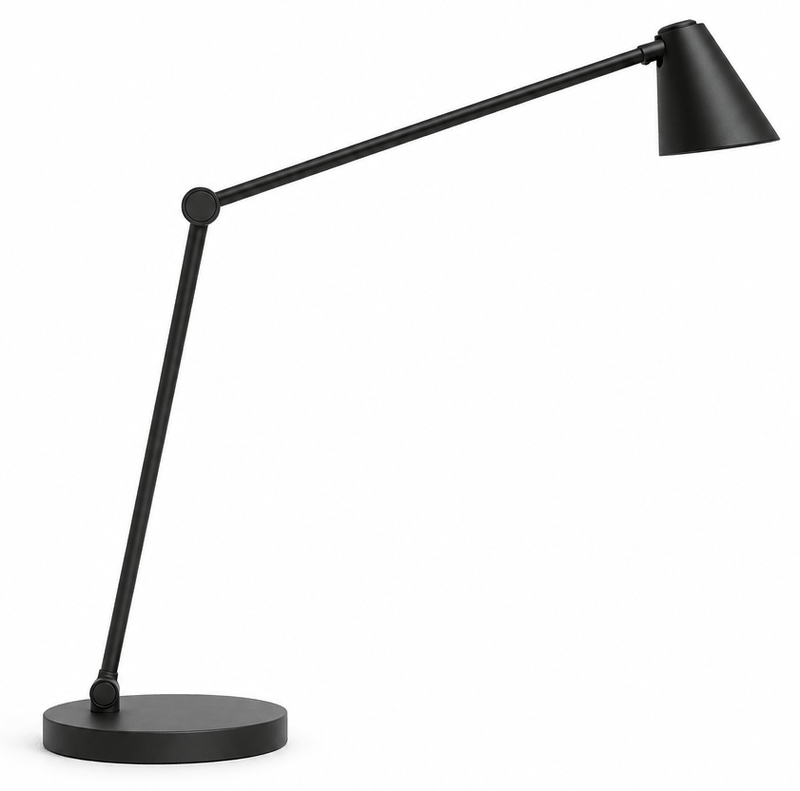
\includegraphics[height=3.2cm]{../scripts/типи_геометрії/nmt_desk_lamp.png}}\\[0.1cm]
\small Рис. 1 & \small Рис. 2
\end{tabular}\end{nmtfit}\end{center}}
\answerTable{$40^\circ$}{$80^\circ$}{$100^\circ$}{$110^\circ$}{$140^\circ$}
\par\penalty-20
\end{samepage}

\begin{samepage}
\zadtask{Розв'яжіть нерівність $0{,}5^{\,x^2-4x}\geqslant 16$.}
\answerTable{$2$}{$(-\infty;\,2]$}{$[2;\,+\infty)$}{розв'язків немає}{$(-\infty;\,+\infty)$}
\par\penalty-20
\end{samepage}

\begin{samepage}
\noindent
\begin{minipage}[c]{0.58\textwidth}
\raggedright\zadnum На рисунку зображено правильну шестикутну призму $ABCDEFA_1B_1C_1D_1E_1F_1$. Скільки всього граней цієї призми лежать у~площинах, \textit{паралельних} прямій $AB$?
\end{minipage}\hfill
\begin{minipage}[c]{0.38\textwidth}\centering
\begin{nmtfit}\begin{tikzpicture}[scale=1.1, line join=round]
\draw[thick] (-1.061,-0.498) -- (0.388,-0.68);
\draw[thick] (0.388,-0.68) -- (1.449,-0.182);
\draw[thick, dashed] (1.449,-0.182) -- (1.061,0.498);
\draw[thick, dashed] (1.061,0.498) -- (-0.388,0.68);
\draw[thick, dashed] (-0.388,0.68) -- (-1.449,0.182);
\draw[thick] (-1.061,-0.498) -- (-1.449,0.182);
\draw[thick] (-1.061,2.327) -- (0.388,2.145);
\draw[thick] (0.388,2.145) -- (1.449,2.643);
\draw[thick] (1.449,2.643) -- (1.061,3.323);
\draw[thick] (1.061,3.323) -- (-0.388,3.506);
\draw[thick] (-0.388,3.506) -- (-1.449,3.008);
\draw[thick] (-1.061,2.327) -- (-1.449,3.008);
\draw[thick] (0.388,-0.68) -- (0.388,2.145);
\draw[thick] (-1.061,-0.498) -- (-1.061,2.327);
\draw[thick] (1.449,-0.182) -- (1.449,2.643);
\draw[thick, dashed] (1.061,0.498) -- (1.061,3.323);
\draw[thick, dashed] (-0.388,0.68) -- (-0.388,3.506);
\draw[thick] (-1.449,0.182) -- (-1.449,3.008);
\draw[mainGreen!65!black, line width=1.8pt] (-1.061,-0.498) -- (0.388,-0.68);
\node[font=\small, inner sep=0pt] at (-1.273,-0.71) {$A$};
\node[font=\small, inner sep=0pt] at (0.414,-0.979) {$B$};
\node[font=\small, inner sep=0pt] at (1.731,-0.285) {$C$};
\node[font=\small, inner sep=0pt] at (0.934,0.226) {$D$};
\node[font=\small, inner sep=0pt] at (-0.378,0.38) {$E$};
\node[font=\small, inner sep=0pt] at (-1.748,0.156) {$F$};
\node[font=\small, inner sep=0pt] at (-0.937,2.708) {$A_1$};
\node[font=\small, inner sep=0pt] at (0.401,2.505) {$B_1$};
\node[font=\small, inner sep=0pt] at (1.808,2.675) {$C_1$};
\node[font=\small, inner sep=0pt] at (1.292,3.599) {$D_1$};
\node[font=\small, inner sep=0pt] at (-0.388,3.806) {$E_1$};
\node[font=\small, inner sep=0pt] at (-1.816,3.106) {$F_1$};
\end{tikzpicture}\end{nmtfit}
\end{minipage}
\par\nbvspace{0.2cm}
\answerTable{одна}{дві}{три}{чотири}{шість}
\par\penalty-20
\end{samepage}

\begin{samepage}
\zadtask{Значення якого з~наведених виразів \textbf{не залежить} від значення змінної $x$?}
\par\nopagebreak\nbvspace{0.1cm}\noindent\begin{tabular}{@{}l@{\quad}l@{}}
\textbf{А} & $(x+3)^2-(x-3)^2$ \\[0.25cm]
\textbf{Б} & $(x-3)(3-x)+x^2$ \\[0.25cm]
\textbf{В} & $(x+3)^2-x(x+3)$ \\[0.25cm]
\textbf{Г} & $(x+3)^2-(x+1)(x+5)$ \\[0.25cm]
\textbf{Д} & $(x-3)^2-(x^2+6x)$
\end{tabular}\par\nbvspace{0.25cm}
\par\penalty-20
\end{samepage}

\begin{samepage}
\zadtask{Укажіть проміжок, якому належить корінь рівняння $\log_2(x+2)+\log_2(x-2)=5$.}
\answerTable{$(-\infty;\,-4)$}{$[-4;\,2)$}{$[2;\,6)$}{$[6;\,10)$}{$[10;\,+\infty)$}
\par\penalty-20
\end{samepage}

\begin{samepage}
\noindent
\begin{minipage}[c]{0.55\textwidth}
\raggedright\zadnum На рисунку зображено графік функції $y=f(x)$, визначеної на проміжку $[-6;\,5]$. Скільки нулів має функція $y=f(x)-2$?
\end{minipage}\hfill
\begin{minipage}[c]{0.41\textwidth}\centering
\begin{nmtfit}\begin{tikzpicture}[scale=0.45]
\draw[gray!35, very thin] (-7,-4) grid (6,5);
\draw[->] (-7,0) -- (6.5,0) node[below left, font=\footnotesize] {$x$};
\draw[->] (0,-4) -- (0,5.5) node[below left, font=\footnotesize] {$y$};
\node[below left, font=\scriptsize] at (0,0) {$0$};
\node[below, font=\scriptsize] at (1,0) {$1$}; \node[left, font=\scriptsize] at (0,1) {$1$};
\draw[very thick] (-6,-3) .. controls (-5.333,0) and (-4.667,2) .. (-4,2) .. controls (-3.333,2) and (-2.667,-1) .. (-2,-1) .. controls (-1.333,-1) and (-0.667,4) .. (0,4) .. controls (1,4) and (2,-1) .. (3,-1) .. controls (3.667,-1) and (4.333,-0.378) .. (5,1);
\node[circle, fill, inner sep=1.5pt] at (-6,-3) {}; \node[circle, fill, inner sep=1.5pt] at (5,1) {};
\end{tikzpicture}\end{nmtfit}
\end{minipage}
\par\nbvspace{0.2cm}
\answerTable{$1$}{$2$}{$3$}{$4$}{$5$}
\par\penalty-20
\end{samepage}

\begin{samepage}
\zadtask{Сторони трикутника дорівнюють $6$~см, $8$~см і~$10$~см. Які з~наведених тверджень про цей трикутник є правильними?\par\nopagebreak\nbvspace{0.1cm}\noindent\begin{tabular}{@{}r@{\ \ }p{0.9\linewidth}@{}}I. & Трикутник прямокутний. \\ II. & Радіус кола, описаного навколо трикутника, дорівнює $5$~см. \\III. & Площа трикутника дорівнює $48$~см$^2$.\end{tabular}}
\answerTable{лише I}{лише III}{лише I та II}{лише II та III}{I, II та III}
\par\penalty-20
\end{samepage}

\begin{samepage}
\zadtask{У~геометричній прогресії $(b_n)$ відомо, що $b_2=16$, $b_5=-2$. Знайдіть суму перших чотирьох членів цієї прогресії.}
\answerTable{$-20$}{$-5$}{$10$}{$40$}{$60$}
\par\penalty-20
\end{samepage}

\begin{samepage}
\zadtask{У~плейлисті Дмитра $20$ треків, з~них $5$ -- його улюбленого гурту. Дмитро вмикає режим «перемішати». Яка ймовірність того, що першим заграє трек улюбленого гурту?}
\answerTableTall{$\dfrac{3}{4}$}{$\dfrac{1}{4}$}{$\dfrac{1}{3}$}{$\dfrac{1}{20}$}{$\dfrac{1}{5}$}
\par\penalty-20
\end{samepage}

\begin{samepage}
\noindent
\begin{minipage}[c]{0.55\textwidth}
\raggedright\zadnum У~прямокутній системі координат у~просторі зображено прямокутний паралелепіпед $ABCDA_1B_1C_1D_1$, вершина $A$ якого збігається з~початком координат, а~ребра $AB$, $AD$ і~$AA_1$ лежать на додатних півосях $x$, $y$ і~$z$ відповідно (див.~рисунок). $AB=4$, $AD=8$, $AA_1=6$. Точка $M$ -- середина ребра $DD_1$.\par\nbvspace{3pt}\noindent Визначте координати вектора $\overrightarrow{BM}$.
\end{minipage}\hfill
\begin{minipage}[c]{0.41\textwidth}\centering
\begin{nmtfit}\begin{tikzpicture}[scale=0.62, line join=round, line cap=round]
\coordinate (A) at (0.000,0.000);
\coordinate (B) at (-1.280,-1.760);
\coordinate (C) at (2.720,-1.760);
\coordinate (D) at (4.000,0.000);
\coordinate (A1) at (0.000,3.000);
\coordinate (B1) at (-1.280,1.240);
\coordinate (C1) at (2.720,1.240);
\coordinate (D1) at (4.000,3.000);
\coordinate (M) at (4.000,1.500);
\coordinate (X) at (-2.176,-2.992);
\coordinate (Y) at (5.100,0.000);
\coordinate (Z) at (0.000,4.100);
\draw[->] (B) -- (X);
\draw[->] (D) -- (Y);
\draw[->] (A1) -- (Z);
\draw[thick, dashed] (A) -- (B);
\draw[thick, dashed] (A) -- (D);
\draw[thick, dashed] (A) -- (A1);
\draw[thick] (B) -- (C) -- (D) -- (D1) -- (A1) -- (B1) -- (B);
\draw[thick] (B1) -- (C1) -- (C);
\draw[thick] (C1) -- (D1);
\draw[-{Stealth[length=5pt]}, thick, dashed, shorten >=2.5pt, mainGreen!60!black] (B) -- (M);
\node[circle, fill, inner sep=1.3pt] at (M) {};
\node[font=\small, inner sep=0pt] at (-0.436,0.252) {$A$};
\node[font=\small, inner sep=0pt] at (-1.716,-1.508) {$B$};
\node[font=\small, inner sep=0pt] at (3.091,-2.131) {$C$};
\node[font=\small, inner sep=0pt] at (4.262,-0.454) {$D$};
\node[font=\small, inner sep=0pt] at (-0.601,3.161) {$A_1$};
\node[font=\small, inner sep=0pt] at (-1.845,1.240) {$B_1$};
\node[font=\small, inner sep=0pt] at (2.264,1.696) {$C_1$};
\node[font=\small, inner sep=0pt] at (4.456,3.456) {$D_1$};
\node[font=\small, inner sep=0pt] at (4.443,1.619) {$M$};
\node[font=\small, inner sep=0pt] at (-2.547,-3.363) {$x$};
\node[font=\small, inner sep=0pt] at (5.100,-0.452) {$y$};
\node[font=\small, inner sep=0pt] at (-0.395,4.100) {$z$};
\end{tikzpicture}\end{nmtfit}
\end{minipage}
\par\nbvspace{0.2cm}
\answerTable{$(-4;\ 8;\ 3)$}{$(4;\ -8;\ -3)$}{$(0;\ 8;\ 3)$}{$(-4;\ 8;\ 6)$}{$(-4;\ 4;\ 3)$}
\par\penalty-20
\end{samepage}

\begin{samepage}
\zadtask{Обчисліть значення виразу $5-4\sin^2\alpha$, якщо $\cos^2\alpha=0{,}3$.}
\answerTable{$2{,}8$}{$2{,}2$}{$3{,}8$}{$0{,}7$}{$-0{,}2$}
\par\penalty-20
\end{samepage}

\begin{samepage}
\noindent
\begin{minipage}[c]{0.55\textwidth}
\raggedright\zadnum На стороні $BC$ прямокутника $ABCD$ вибрано точку $K$ так, що $\angle AKD=90^\circ$, $\angle KDA=30^\circ$ (див.~рисунок), $AB=4\sqrt3$~см. Знайдіть площу трикутника $AKD$.
\end{minipage}\hfill
\begin{minipage}[c]{0.41\textwidth}\centering
\begin{nmtfit}\begin{tikzpicture}[scale=0.3, line join=round, line cap=round]
\coordinate (A) at (0.000,0.000);
\coordinate (B) at (0.000,6.928);
\coordinate (C) at (16.000,6.928);
\coordinate (D) at (16.000,0.000);
\coordinate (K) at (4.000,6.928);
\draw[thick] (A) -- (B) -- (C) -- (D) -- cycle;
\draw[thick] (A) -- (K) -- (D);
\node[circle, fill, inner sep=1.3pt] at (A) {};
\node[circle, fill, inner sep=1.3pt] at (B) {};
\node[circle, fill, inner sep=1.3pt] at (C) {};
\node[circle, fill, inner sep=1.3pt] at (D) {};
\node[circle, fill, inner sep=1.3pt] at (K) {};
\pic[draw, angle radius=0.2cm] {right angle = A--K--D};
\pic[draw, angle radius=0.45cm] {angle = K--D--A};
\node[font=\small, inner sep=0pt] at (12.108,0.757) {$30^\circ$};
\node[font=\small, inner sep=0pt] at (-0.900,-0.520) {$A$};
\node[font=\small, inner sep=0pt] at (-0.900,7.448) {$B$};
\node[font=\small, inner sep=0pt] at (16.900,7.448) {$C$};
\node[font=\small, inner sep=0pt] at (16.900,-0.520) {$D$};
\node[font=\small, inner sep=0pt] at (4.267,7.924) {$K$};
\end{tikzpicture}\end{nmtfit}
\end{minipage}
\par\nbvspace{0.2cm}
\answerTable{$16\sqrt3$~см$^2$}{$64\sqrt3$~см$^2$}{$24\sqrt3$~см$^2$}{$32\sqrt3$~см$^2$}{$48$~см$^2$}
\par\penalty-20
\end{samepage}

\begin{samepage}
\zadtask{Пара чисел $(x_0;\,y_0)$ -- розв'язок системи рівнянь \[\begin{cases}x^2y=12,\\ xy^2=18.\end{cases}\] Знайдіть добуток $x_0\cdot y_0$.}
\answerTable{$6\sqrt6$}{$72$}{$216$}{$1{,}5$}{$6$}
\par\penalty-20
\end{samepage}

\instructionBox{У завданнях 16--18 до кожного з трьох рядків інформації, позначених цифрами, доберіть один правильний, на Вашу думку, варіант, позначений буквою.}

\begin{samepage}
\zadtask{Нехай $x=\sqrt{3}-2$. Установіть відповідність між виразом \mbox{(1--3)} та його значенням \mbox{(А--Д)}.}
\nmtnobreak
\nopagebreak\nbvspace{0.3cm}
\noindent
\matchingLayout{
\matchHead{Вираз}
\matchItem{1}{$(x+2)^{-2}$}
\matchItem{2}{$\dfrac{1}{x}$}
\matchItem{3}{$|x|\cdot(x+4)$}
}{
\matchHead{Значення виразу}
\matchItem{А}{$-2-\sqrt{3}$}
\matchItem{Б}{$-1$}
\matchItem{В}{$\dfrac{1}{3}$}
\matchItem{Г}{$1$}
\matchItem{Д}{$3$}
}{
\matchingGrid
}
\par\penalty-20
\end{samepage}

\begin{samepage}
\zadtask{Установіть відповідність між функцією \mbox{(1--3)} та її властивістю \mbox{(А--Д)}.}
\nmtnobreak
\nopagebreak\nbvspace{0.3cm}
\noindent
\matchingLayout{
\matchHead{Функція}
\matchItem{1}{$y=x^2-4$}
\matchItem{2}{$y=\sqrt{x-2}$}
\matchItem{3}{$y=5-2x$}
}{
\matchHead{Властивість функції}
\matchItem{А}{функція парна}
\matchItem{Б}{функція непарна}
\matchItem{В}{функція спадає на $(-\infty;\,+\infty)$}
\matchItem{Г}{$D(y)=[2;\,+\infty)$}
\matchItem{Д}{$E(y)=[2;\,+\infty)$}
}{
\matchingGrid
}
\par\penalty-20
\end{samepage}

\begin{samepage}
\noindent
\begin{minipage}[c]{0.55\textwidth}
\raggedright\zadnum У~паралелограмі $ABCD$ висота $BH$, проведена до сторони $AD$, ділить її на відрізки $AH=5$~см і~$HD=11$~см, $BH=12$~см (див.~рисунок). Установіть відповідність між фігурою \mbox{(1--3)} та її площею \mbox{(А--Д)}.
\end{minipage}\hfill
\begin{minipage}[c]{0.41\textwidth}\centering
\begin{nmtfit}\begin{tikzpicture}[scale=0.2, line join=round, line cap=round]
\coordinate (A) at (0.000,0.000);
\coordinate (B) at (5.000,12.000);
\coordinate (C) at (21.000,12.000);
\coordinate (D) at (16.000,0.000);
\coordinate (H) at (5.000,0.000);
\draw[thick] (A) -- (B) -- (C) -- (D) -- cycle;
\draw[thick, dashed] (B) -- (H);
\node[circle, fill, inner sep=1.3pt] at (A) {};
\node[circle, fill, inner sep=1.3pt] at (B) {};
\node[circle, fill, inner sep=1.3pt] at (C) {};
\node[circle, fill, inner sep=1.3pt] at (D) {};
\node[circle, fill, inner sep=1.3pt] at (H) {};
\pic[draw, angle radius=0.2cm] {right angle = B--H--D};
\node[font=\small, inner sep=0pt] at (-1.351,-0.780) {$A$};
\node[font=\small, inner sep=0pt] at (3.649,12.780) {$B$};
\node[font=\small, inner sep=0pt] at (22.351,12.780) {$C$};
\node[font=\small, inner sep=0pt] at (17.351,-0.780) {$D$};
\node[font=\small, inner sep=0pt] at (4.600,-1.493) {$H$};
\end{tikzpicture}\end{nmtfit}
\end{minipage}\par
\nmtnobreak
\nopagebreak\nbvspace{0.3cm}
\noindent
\matchingLayout{
\matchHead{Фігура}
\matchItem{1}{трикутник $ABH$}
\matchItem{2}{паралелограм $ABCD$}
\matchItem{3}{трапеція $HBCD$}
}{
\matchHead{Площа}
\matchItem{А}{$30$~см$^2$}
\matchItem{Б}{$60$~см$^2$}
\matchItem{В}{$96$~см$^2$}
\matchItem{Г}{$162$~см$^2$}
\matchItem{Д}{$192$~см$^2$}
}{
\matchingGrid
}
\par\penalty-20
\end{samepage}

\instructionBox{Розв'яжіть завдання 19--22. Одержані числові відповіді запишіть у бланку відповідей. Відповідь записуйте лише десятковим дробом, урахувавши положення коми. Знак «мінус» записуйте перед першою цифрою числа.}

\begin{samepage}
\zadtask{Водій помітив на дорозі перешкоду й~почав гальмувати. Шлях $s$ (у~метрах), який автомобіль проїхав за $t$~секунд від початку гальмування, змінювався за законом $s(t)=20t-2t^2$. Скільки метрів проїхав автомобіль від початку гальмування до повної зупинки?}
\nmtnobreak
\nopagebreak\nbvspace{0.4cm}
\nmtAnswerBox
\par\penalty-20
\end{samepage}

\begin{samepage}
\zadtask{Марта написала п'ять пробних НМТ з~математики. Її результати (у~балах за шкалою $100$--$200$) наведено в~таблиці. Після шостого пробного НМТ середній результат Марти (уже за всі шість пробних) зріс на $4$~бали. Скільки балів Марта отримала за \textit{шостий} пробний НМТ?\par\nopagebreak\nbvspace{0.15cm}\noindent\begin{center}\renewcommand{\arraystretch}{1.3}\begin{tabular}{|l|*{5}{>{\centering\arraybackslash}p{0.9cm}|}}\hline \textbf{Пробний НМТ} & 1-й~& 2-й~& 3-й~& 4-й~& 5-й~\\ \hline \textbf{Результат (бали)} & $152$ & $160$ & $148$ & $171$ & $164$ \\ \hline\end{tabular}\end{center}}
\nmtnobreak
\nopagebreak\nbvspace{0.4cm}
\nmtAnswerBox
\par\penalty-20
\end{samepage}

\begin{samepage}
\zadtask{На рисунку зображено тіло, складене з~правильної чотирикутної призми й~правильної чотирикутної піраміди, основа якої збігається з~верхньою основою призми. Сторона основи призми дорівнює $6$~см, висота призми~-- $8$~см, а~бічні грані піраміди нахилені до площини її основи під кутом $60^\circ$. Визначте площу (у~см$^2$) поверхні тіла.}
\nmtnobreak
\nopagebreak\nbvspace{0.3cm}
\begin{center}\begin{nmtfit}\begin{tikzpicture}[scale=1.1, line join=round]
\begin{scope}[shift={(0,0)}]
\draw[thick] (-1.366,-0.155) -- (0.366,-0.577);
\draw[thick] (0.366,-0.577) -- (1.366,0.155);
\draw[thick, dashed] (1.366,0.155) -- (-0.366,0.577);
\draw[thick, dashed] (-1.366,-0.155) -- (-0.366,0.577);
\draw[thick] (0.366,-0.577) -- (0.366,1.843);
\draw[thick] (-1.366,2.265) -- (0.366,1.843);
\draw[thick] (-1.366,-0.155) -- (-1.366,2.265);
\draw[thick] (1.366,0.155) -- (1.366,2.575);
\draw[thick] (0.366,1.843) -- (1.366,2.575);
\draw[thick, dashed] (-0.366,0.577) -- (-0.366,2.997);
\draw[thick, dashed] (1.366,2.575) -- (-0.366,2.997);
\draw[thick, dashed] (-1.366,2.265) -- (-0.366,2.997);
\draw[thick] (0.366,1.843) -- (0,3.988);
\draw[thick] (-1.366,2.265) -- (0,3.988);
\draw[thick] (1.366,2.575) -- (0,3.988);
\draw[thick, dashed] (-0.366,2.997) -- (0,3.988);
\end{scope}
\end{tikzpicture}\end{nmtfit}\end{center}
\nmtnobreak
\nopagebreak\nbvspace{0.4cm}
\nmtAnswerBox
\par\penalty-20
\end{samepage}

\begin{samepage}
\zadtask{Визначте \textit{суму} всіх цілих значень $a$, за кожного з~яких рівняння \[\dfrac{4^{x-a}-2^{x-a+1}-8}{\sqrt{25-x^2}}=0\] має корінь.}
\nmtnobreak
\nopagebreak\nbvspace{0.4cm}
\nmtAnswerBox
\par\penalty-20
\end{samepage}

\end{document}
